\documentclass{article}
\usepackage{verbatim,fancyvrb}
\usepackage{pifont}
%\usepackage[authoryear]{natbib}
\usepackage[pdftex]{graphicx}
\usepackage{gretl}
\usepackage[hyphens]{url}
\usepackage{hyperref}
\usepackage[letterpaper,body={6.3in,9.15in},top=.8in,left=1.1in]{geometry}

\setlength{\parindent}{0pt}
\setlength{\parskip}{1ex}
\setlength{\abovecaptionskip}{0pt}

\title{geoplot: cartography in gretl}
\author{Allin Cottrell and Jack Lucchetti}

\begin{document}

\maketitle

\textbf{Warning}: As of this writing the \textsf{geoplot} package is
in ``alpha'' mode (or at best ``beta''). You're welcome to try it, but
expect some bugs, and do not bank on the user interface remaining
unchanged.

That said, section~\ref{sec:prelim} below covers some preliminaries
which we hope will help the reader to understand what's going
on. Section~\ref{sec:workflow} describes the basic workflow for
producing a map image via gretl. Section~\ref{sec:example} then
provides a simple worked example and section~\ref{sec:pairing}
addresses a potential stumbling block. Section~\ref{sec:opts} goes
over the current options to the core \texttt{geoplot} function in
detail; section~\ref{sec:expert} explains some ``expert'' refinements;
and section~\ref{sec:future} gives our current thinking on possible
future directions for maps in gretl.

\section{Preliminaries}
\label{sec:prelim}

Given gretl's user base and vocation, we assume that people will be
primarily interested in ``thematic'' maps, in which geographical areas
get different colors according to some variable of interest (for
example regions of a country are colored according to their
unemployment rates). Fancier maps are out of scope for the
present. From here on we'll simply refer to maps of this sort as
``maps'' and the geographical entities they contain (which may be
countries, states, counties, l\"ander or whatever) as
``regions''. Plotting a map typically involves drawing a number of
polygons, filled with appropriate colors, to some device (the screen,
or a file).\footnote{One may want to draw colored lines, such as
  rivers or roads: not for now.}

The essential ingredients for doing this are
\begin{enumerate}
   \item A geometrical description of the regions.
   \item The data for coloring the polygons.
   \item Appropriate software for producing the map.
\end{enumerate}

\subsection{The geometry}
\label{sec:geometry}

Let's say we have $n$ regions, indexed by $i$. Region $i$ is
represented geometrically as a collection of $k_i$ polygons (think
islands in an archipelago), indexed by $j$. Each polygon is defined by
$h_{i,j}$ coordinates. Typically, each coordinate vector has two
elements, latitude and longitude.\footnote{In some cases you may have
  a third element---altitude being the most obvious candidate---or
  more.  But we're not getting into that right now.}

The information on each region has two components:
\begin{description}
\item[Metadata] At minimum this should include the region's
  identifier(s), as strings and/or numerical codes. Other information,
  such as land area, may also be included. You can think of this as a
  dataset with $n$ observations and several variables, possibly
  string-valued.
\item[Polygons] A representation of the region's shape on the map, in
  the form of one or more polygons, each taking the form of an array
  of X--Y pairs, typically latitude and longitude. You can think of
  this as an array of arrays of 2-column matrices: the outer array is
  of size $n$; inner array $i$ contains $k_i$ matrices, each with two
  columns.
\end{description}

Several file formats can be used for storing the geometry
information.\footnote{The site
\url{https://ec.europa.eu/eurostat/web/gisco/geodata/reference-data/administrative-units-statistical-units/nuts}
offers a nice collection for European NUTS regions (NUTS =
Nomenclature of Territorial Units for Statistics).}
Gretl supports what are probably the two most common formats:
\begin{itemize}
\item GeoJSON files: plain JSON files with a pre-specified internal
  structure, regulated by RFC 7946. Basically, an array of regions (or
  ``features'') with each element containing the metadata and the
  polygons, under the \texttt{properties} and \texttt{geometry} keys,
  respectively.  This is our preferred format.\footnote{In the future
    we may take a look at an evolution of GeoJSON called TopoJSON, but
    that's not a priority at the moment.}
\item ESRI shapefiles: more of a ``legacy'' format, but still very
  common in the wild. These maps come as collections of several files,
  usually zipped together. The essential components are an
  \textsf{xBase} file, with \texttt{dbf} extension, holding the
  metadata; the shapefile proper with extension \texttt{shp}, holding
  the polygons; and an index file with extension \texttt{shx}, used
  to speed up operations when reading the data.
\end{itemize}

\subsection{The payload data}
\label{sec:payload}

By ``payload'' we mean the data used for coloring the regions.  We
assume that the payload is available as a gretl series. This typically
means that the user has a data file (in native \texttt{gdt} format or
some other format gretl can read) in which each line represents a
region, as illustrated in Table~\ref{tab:payload}. Note in particular
the ``id'' column.  We assume that the map metadata contain sufficient
information to establish a correspondence with the dataset containing
the payload: either a numerical code or a suitable string-valued
variable.  One thing one quickly learns in exploring a variety of
\texttt{geojson} and \texttt{shp} files is that there's no telling how
the regions will be ordered; one \textit{cannot} assume that they
occur in what one might think of as ``standard'' order (e.g.\
alphabetical order for US states).

\begin{table}[htbp]
\begin{center}
\begin{tabular}{llrr}
  %\hline
  id	& State & Pop2019 & Pop2010 \\
  \hline \\ [-1.75ex]
  1	& Alabama	& 4903185	& 4779736  \\
  2     & Alaska	& 731545	& 710231   \\
  101   & American Samoa	& 55641	& 55519	  \\
  3	& Arizona	& 6278717	& 6392017  \\
  4	& Arkansas	& 3017825	& 2915918  \\
  5	& California	& 39512223	& 37254523 \\
  6	& Colorado	& 5758736	& 5029196  \\
  7	& Connecticut	& 3565287	& 3574097  \\
                & \vdots & \\
  %\hline
\end{tabular}
\end{center}
\caption{Typical format for a payload dataset}
\label{tab:payload}
\end{table}


\subsection{The software backend}
\label{sec:software}

In principle one could represent maps using any one of the many
plotting libraries around, but gretl uses \textsf{gnuplot}, which we
already use for all other kinds of plot. Details on the
\textsf{gnuplot} commands we use can be found in
Appendix~\ref{sec:gnuplot}.

Given the geometry data and the payload, writing a \textsf{gnuplot}
script for producing the map is straightforward. And in most cases
\textsf{gnuplot} can produce a plot in short order. You might have to
wait a little if there are many regions, of complex shapes,
represented in high precision in the source map file.

\section{The workflow}
\label{sec:workflow}

Typical workflow for producing a thematic map in gretl is likely to be
as follows.

\begin{enumerate}
\item You \cmd{open} the map-datafile as a gretl dataset; this reads
  in the metadata so gretl's \dollar{nobs} will be equal to the number
  of regions, $n$.
\item You add the payload data, via the \texttt{append} or
  \texttt{join} commands or in some other way.
\item You decide on some details of your map (appearance, format,
  etc.), with sensible defaults being available.
\item Finally, you create the map.
\end{enumerate}

Point 1 is handled by using the existing \texttt{open} command on the
map-datafile. The filename extensions recognized for this purpose are
\texttt{json} or \texttt{geojson} for GeoJSON files, \texttt{dbf} or
\texttt{shp} for ESRI shapefiles.\footnote{In principle we could read
  the polygons at this point and store them in RAM, but for now we
  don't. We just read in the metadata, but store the path to the
  associated geometry file internally; we could provide an accessor
  for this path (\dollar{mapdata}?) but we're not doing that yet. A
  possible future development is to make all the map information
  (metadata and polygons) available as a gretl bundle under a suitable
  accessor.} Point 2 is also handled by existing gretl commands.

As for points 3 and 4, these are currently handled by the new
(built-in) \texttt{geoplot} function.\footnote{At some point
  production of maps may be supported by a gretl command, either in
  its own right or as a variant of the existing \texttt{plot}
  command.} This function has this signature:
\begin{code}
function void geoplot(const string mapfile,
	              const series payload[null],
	              const bundle options[null])
\end{code}
Here \texttt{mapfile} is the (required) name of the file containing
the polygons, \texttt{payload} is the (optional) series with which to
colorize the polygons, and \texttt{options} is an (optional) bundle to
contain one or more elements governing the appearance or destination
of the plot.

[MOVE? If the \cmd{geoplot} call follows on the opening of a map metadata
file in the same session, the \texttt{mapfile} argument may be
regarded as already implicit (it will be the very same file in the
GeoJSON case, or an shp file with the same basename as a previously
opened dbf file), but for now we're requiring that its path be given.]

[MOVE? If the \texttt{payload} argument is given as \texttt{null} or omitted
then the map is drawn ``as is'', without any colorization. This can be
useful if you just want to see what a geometry file looks like.]

If the \texttt{options} bundle is omitted all options are set to their
default values. The keys that are currently handled in the options
bundle are listed (along with their default values) in section
\ref{sec:opts}.

\section{An example}
\label{sec:example}

For this example we'll produce a map showing GDP per capita of the six
founder countries of the EU, using three files: script
\texttt{founders.inp}, data file \texttt{founders.csv} and map
\texttt{founders.geojson}. In this case the required files are small
enough to be readily inspected by hand.  The content of
\texttt{founders.csv}, which holds what will be the payload, is shown
in Listing~\ref{tab:founders-csv}.

\begin{script}[htbp]
\begin{scode}
Name,code,pop,area,gdp
Belgium,BE,11365834,30528,534230
France,FR,67024633,632833,2833687
Germany,DE,82437641,357386,3874437
Italy,IT,61219113,301338,2147744
Luxembourg,LU,589370,2586.4,65683
Netherlands,NL,17220721,41543,880716
\end{scode}
\caption{Content of \texttt{founders.csv}}
\label{tab:founders-csv}
\end{script}

\begin{script}[htbp]
  \begin{scode}
{"type": "FeatureCollection", "features": [
 {"geometry": {"type": "Polygon", "coordinates": [[[40.40360,
     30.79039], [40.59686, 30.49366], [40.65087, 30.29746], ... ]]},
   "type": "Feature", "properties": {"CNTR_NAME": "Belgique",
     "ISO3_CODE": "BEL", "CNTR_ID": "BE", "NAME_ENGL": "Belgium",
     "FID": "BE"}, "id": "BE"},
 {"geometry": {"type": "MultiPolygon", "coordinates": [[[[40.18497,
     29.45664], [40.23634, 29.39875], [40.57754, 29.35021], ...],
     [[[42.66689, 20.70300], [42.57348, 20.41660], ...]]},
   "type": "Feature", "properties": {"CNTR_NAME": "France",
     "ISO3_CODE": "FRA", "CNTR_ID": "FR", "NAME_ENGL": "France",
     "FID": "FR"}, "id": "FR"},
  ...
\end{scode}
\caption{Excerpt of \texttt{founders.geojson}}
\label{tab:json-xrpt}
\end{script}

The JSON file is too big to show here in full but small enough to
examine in any text editor.\footnote{Even Microsoft's
  \texttt{Notepad}!} Listing~\ref{tab:json-xrpt} contains a
representative excerpt. Note that while Belgium is a single polygon
France is an array of polygons (``\texttt{MultiPolygon}''), because of
Corsica.

\begin{script}[htbp]
\begin{scode}
open founders.geojson

join founders.csv gdp pop --ikey=FID --okey=code
series gdppc = 1000*gdp/pop

opts = defbundle("plotfile", "GDPpc.plt", "inlined", 1)
geoplot($mapfile, gdppc, opts)
\end{scode}
  %$
\caption{Content of \texttt{founders.inp}}
\label{tab:founders-script}
\end{script}

The \texttt{founders.inp} script is shown in
Listing~\ref{tab:founders-script}, and what we get after opening the
\texttt{geojson} file in gretl is in Listing~\ref{tab:founders-meta}.

\begin{script}[htbp]
\begin{scode}
     CNTR_NAME    ISO3_CODE      CNTR_ID    NAME_ENGL          FID

1     Belgique          BEL           BE      Belgium           BE
2       France          FRA           FR       France           FR
3  Deutschland          DEU           DE      Germany           DE
4       Italia          ITA           IT        Italy           IT
5    Luxemburg          LUX           LU   Luxembourg           LU
6    Nederland          NLD           NL  Netherlands           NL
\end{scode}
\caption{The ``founders'' metadata}
\label{tab:founders-meta}  
\end{script}

Next, we perform the \cmd{join} with \texttt{FID} (from the JSON file)
as the inner key and \texttt{code} (from the CSV file) as the outer
key. Finally, we call the \cmd{geoplot} function to create an
on-screen map. We specify the \texttt{mapfile} to use and the
\texttt{payload} to colorize. Via the \texttt{options} argument we add
a couple of points: the \textsf{gnuplot} input file should be saved
under the name \texttt{GDPpc.plt}, and the geometry data should be
``inlined'' in this file, making it self-contained.

Running the script will produce a gnuplot file like the following:

\begin{code}
set term wxt persist

unset key
set cbrange [33.3288:117.018]
set xrange [31.7826:51.4213]
set yrange [14.7701:36.0553]
$MapData << EOD
40.4036 30.79039 47.00315
40.59686 30.49366 47.00315

[...]

38.92268 31.40258 51.142806
38.59809 31.50169 51.142806
38.59737 31.60855 51.142806

EOD
plot for [i=0:*] $MapData index i with filledcurves fc palette, \
  $MapData using 1:2 with lines lc "white" lw 1
\end{code}
%$

and feeding the above into \textsf{gnuplot} yields the map shown in
Figure~\ref{fig:founders}.

\begin{figure}[htbp]
  \begin{center}
  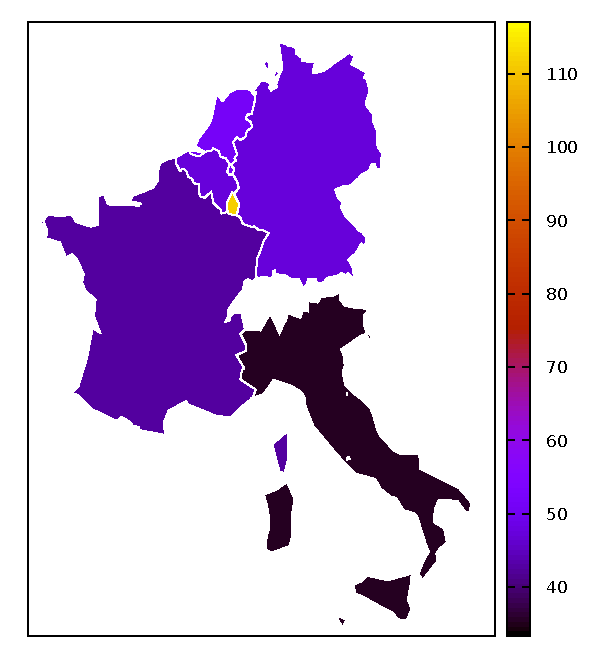
\includegraphics[scale=0.9]{GDPpc.pdf}
\end{center}
\caption{Output of script \texttt{founders.inp}}
\label{fig:founders}
\end{figure}


\section{The pairing problem}
\label{sec:pairing}

There's a potential problem with the strategy outlined above: possible
decoupling of the metadata loaded via \cmd{open} and the geometry data
loaded via the \texttt{geoplot} function.

Production of a correct map requires 1:1 correspondence between the
regions represented in the current dataset and those in the geometry
file. This correspondence may be broken by sorting or subampling of
the dataset; in either case observation $i$ in the dataset will no
longer match up with region $i$ in the geometry file. Sorting would be
an unlikely (not to say silly) operation in this context but
subsampling is important, because in some cases one wants to produce a
map that shows only a subset of the available regions. A typical case
is the USA, where you often want to leave out Hawaii, and maybe Alaska
too.

The solution we have at present for subsampling is illustrated in
Listing~\ref{tab:USA}: we create a dummy ``mask'' series, with value 1
for the observations (regions) we wish to exclude, 0 otherwise, and
pass it (in matrix form) to the \texttt{geoplot} function via the
\texttt{options} bundle. Figure~\ref{fig:USA} shows the results with
and without exclusion of Alaska and Hawaii.\footnote{Given the role
  of this example we don't bother adding a real payload, but just
  simulate data using the \texttt{normal} function.}

\begin{script}[p]
  \begin{scode}
open "us-states.geojson" --quiet
x = normal() # fake up some data!
opts = defbundle("plotfile", "us0.plt", "inlined", 1)

# show the entire USA
opts.title = "USA (complete)"
geoplot($mapfile, x, opts)

# skip Alaska and Hawaii
series mask = (postal == "AK" || postal == "HI")
opts.title = "USA (mainland)"
opts.plotfile = "us1.plt"
opts.mask = {mask}
geoplot($mapfile, x, opts)
  \end{scode}
  \caption{US maps (complete vs mainland)}
  \label{tab:USA}
\end{script}

\begin{figure}[p]
  \begin{center}
  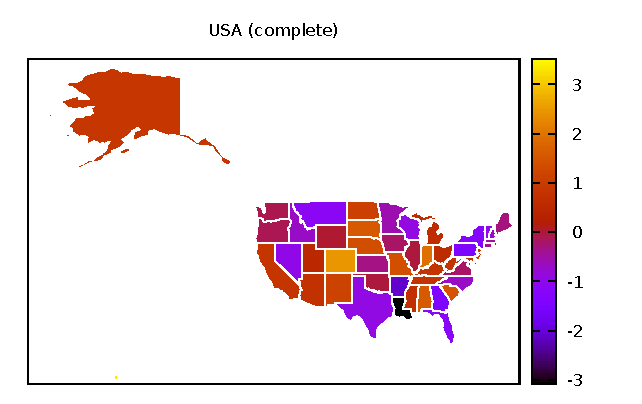
\includegraphics[scale=0.9]{us0.pdf}

  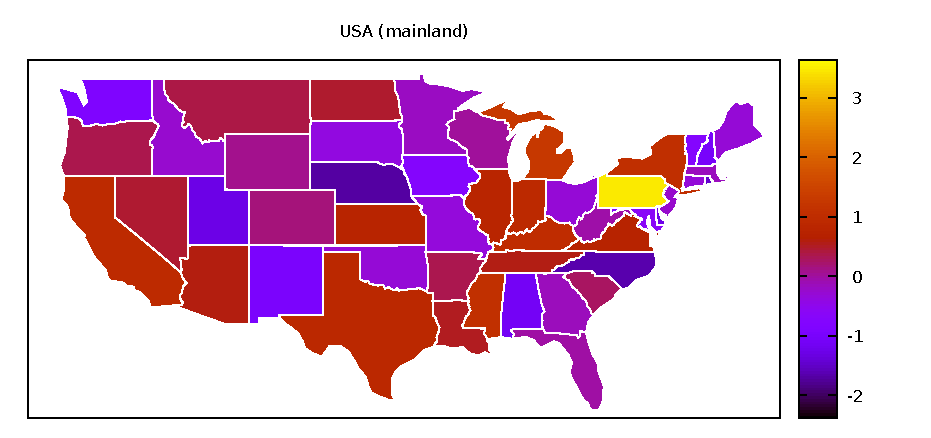
\includegraphics[scale=0.9]{us1.pdf}
\end{center}
\caption{Output of Listing \ref{tab:USA}}
\label{fig:USA}
\end{figure}

A related but different problem arises when the map data and the
payload come from different sources, as they usually will. In this
case, there may be a problem of \texttt{join}ing the regions correctly
if discrepancies arise between the inner and outer keys. But this
problem is not specific to the mapping apparatus, it's a more general
issue concerning the matching of data from different sources, and we
need not be concerned with it here.

\section{Options for the \texttt{geoplot} function}
\label{sec:opts}

We first present all the currently supported options in alphabetical
order. Below the listing we give some further explanation of the usage
of \texttt{plotfile}, \texttt{show} and \texttt{inlined}.

\begin{description}
\item[\texttt{bordwidth}:] scalar, thickness of the line used for the
  borders of the regions: Default: 1.
\item[\texttt{height}:] scalar, giving the height of the plot (in
  pixels for PNG output, which is the only case handled so far). If
  this is given we try to figure out the width which gives a suitable
  aspect ratio for the plot and write these dimensions into the plot
  file. Default: 600.
\item[\texttt{inlined}:] Boolean, to have the polygon data included
  directly into the gnuplot file. Default: false, the data are read
  from a separate file.
\item[\texttt{logscale}:] Boolean, use log scale for the
  payload. Default: false.
\item[\texttt{mask}:] a column vector of length equal to the number of
  features in the map, with zeros in all places other than features to
  be excluded, which should be represented by \texttt{NA}s. This is
  very much a provisional formulation and should be improved. The mask
  is referenced only if \texttt{payload} is not provided; it provides
  an alternative means of subsetting the features. Default: none.
\item[\texttt{tics}:] Boolean, for turning on the printing of x
  (longitude) and y (latitude) tics. Default: tics are suppressed,
  unless \texttt{geoplot()} is invoked without any payload or option
  bundle.
\item[\texttt{plotfile}:] filename, allowing the user to direct output
  of the generated gnuplot command file. We recommend using the
  extension ``\texttt{.plt}'' for such files. If \texttt{plotfile} is
  given, but not as a full path, the file is written to the user's
  working directory. By default the command file is written to the
  user's ``dotdir'' (where it will be deleted on exit from gretl).
\item[\texttt{setpal}:] string, giving either a \textsf{gnuplot}
  \texttt{set palette} command or a predefined palette option, of
  which there are currently just two, \texttt{blues} and
  \texttt{oranges}. For example, the syntax
  \begin{code}
    options.setpal = "set palette defined (0 '#D4E4F2', 1 'steelblue')"
  \end{code}
  will give you a pleasant blue gradient---which also happens to be
  what you get by giving
  \begin{code}
    options.setpal = "blues"
  \end{code}
  If no such string is given you get the default built-in
  \textsf{gnuplot} palette.
\item[\texttt{show}:] Boolean, should the plot should be shown
  on-screen right away? Default: true. (Otherwise a gnuplot file is
  written but not displayed.)
\item[\texttt{title}:] string specifying a title for the
  plot. Default: no title.
\end{description}

As regards the output from \texttt{geoplot()} you have these basic
options:
\begin{itemize}
\item Show the map on-screen then discard the file(s) that were used
  to generate the image. This is the default if you do not specify
  \texttt{plotfile} in the options bundle.
\item Show the map on-screen and save the files(s) that generated it.
  This happens if you specify \texttt{plotfile} and do not override
  the default (true) value of \texttt{show}.
\item Don't show anything on-screen, just write file(s) that can be
  used to generate a map via gnuplot. You get this if you specify
  \texttt{plotfile} and set \texttt{show} to 0.
\end{itemize}

Note that if you set \texttt{show} to 0 and do \textit{not} specify
\texttt{plotfile} that is tantamount to saying ``Don't do anything!'',
which is regarded as an error.

A few more words on \texttt{inlined}: \textsf{geoplot} can pass the
map coordinates to gnuplot either by writing them directly into the
commands file (\texttt{inlined} = 1), or by writing them to a separate
data file whose name is recorded in the commands file
(\texttt{inlined} = 0).

The advantage of having the data inlined is that, being all in one
file, the information required to generate a map cannot easily become
``unstuck''. The disadvantage is that the gnuplot command file is
likely to be very large and perhaps not so easy to edit; besides the
gnuplot commands it may contain many thousands of lines of coordinate
data (which in general should \textit{not} be touched, on pain of
breaking the map). At present we have \texttt{inlined} set to 0 by
default but that may change; we recommend making an explicit choice
via the options bundle.

If you specify \texttt{plotfile} but not \texttt{inlined} you'll get
two output files in your working directory: the specified command file
plus a data file named by switching the extension of \texttt{plotfile}
to ``\texttt{.dat}''. For example you might get \texttt{mygeo.plt} and
\texttt{mygeo.dat}; with \texttt{inlined} = 1 you'd just get a big
\texttt{mygeo.plt}.

\section{``Expert'' refinements}
\label{sec:expert}

To be written. Talk about opening GeoJSON or shp files as gretl
bundles, editing in various ways, and saving as GeoJSON. (New
functionality of bread()/bwrite().)

\section{Future directions?}
\label{sec:future}

To be written. Talk about a possible ``command block'' version of
geoplot. Maybe automatic opening of polygons as a bundle when you open
the map metadata. Maybe have smpl handle sub-sampling of regions
without requiring the user to pass a mask. Adding other features to
maps (region names, cities, rivers)? TopoJSON?


\clearpage
\appendix

\section{Representation of polygons in gnuplot}
\label{sec:gnuplot}

The
following \texttt{gnuplot} code
\begin{code}
  unset key
  plot '-' using 1:2:3 with filledcurves fillcolor "blue"
  0 0 0
  0.5 0 0.866
  1 0 0
  e
\end{code}
produces an equilateral triangle: 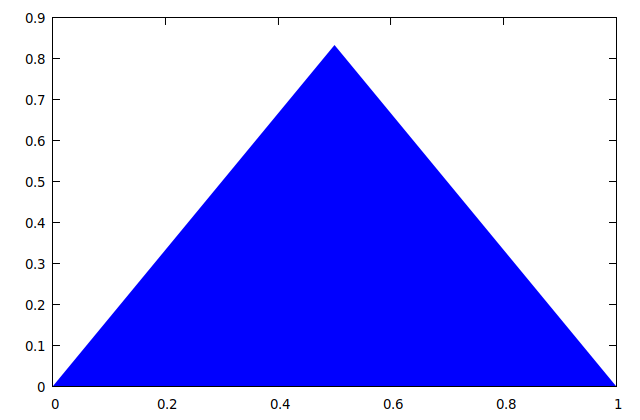
\includegraphics[height=2cm]{triangle.png}

\medskip

The internal coloring of each polygon can be set by using the
\texttt{fillcolor palette} syntax. For example,
\begin{scriptsize}
\begin{code}
unset key
plot for [i=0:*] '-' index i with filledcurves fillcolor palette
	0 0 2.5
	0 1 2.5
	1 1 2.5
	1 0 2.5

	2 1 3.5
	2 2 3.5
	3 2 3.5
	3 1 3.5

	4 0 3
	4 1 3
	5 1 3
	5 0 3

e
e
e
\end{code}
\end{scriptsize}
produces
\begin{center}
  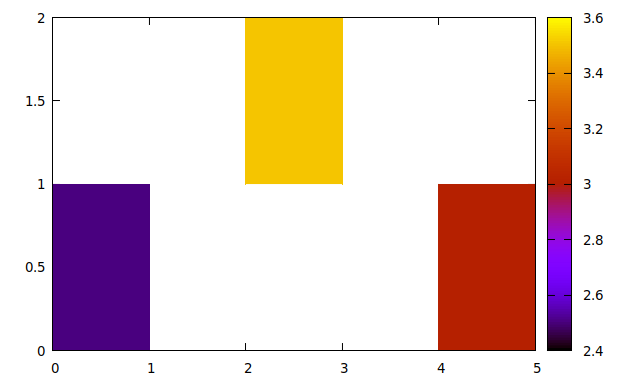
\includegraphics[width=0.6\textwidth]{squares}
\end{center}

A nice way to customize the palette is by using the syntax \texttt{set
palette defined} (see the gnuplot manual).

\end{document}

%%% Local Variables:
%%% mode: latex
%%% TeX-master: t
%%% End:
